% AUTO-GENERATED by code/figlib.py helpers -- do not edit
\nTenFit{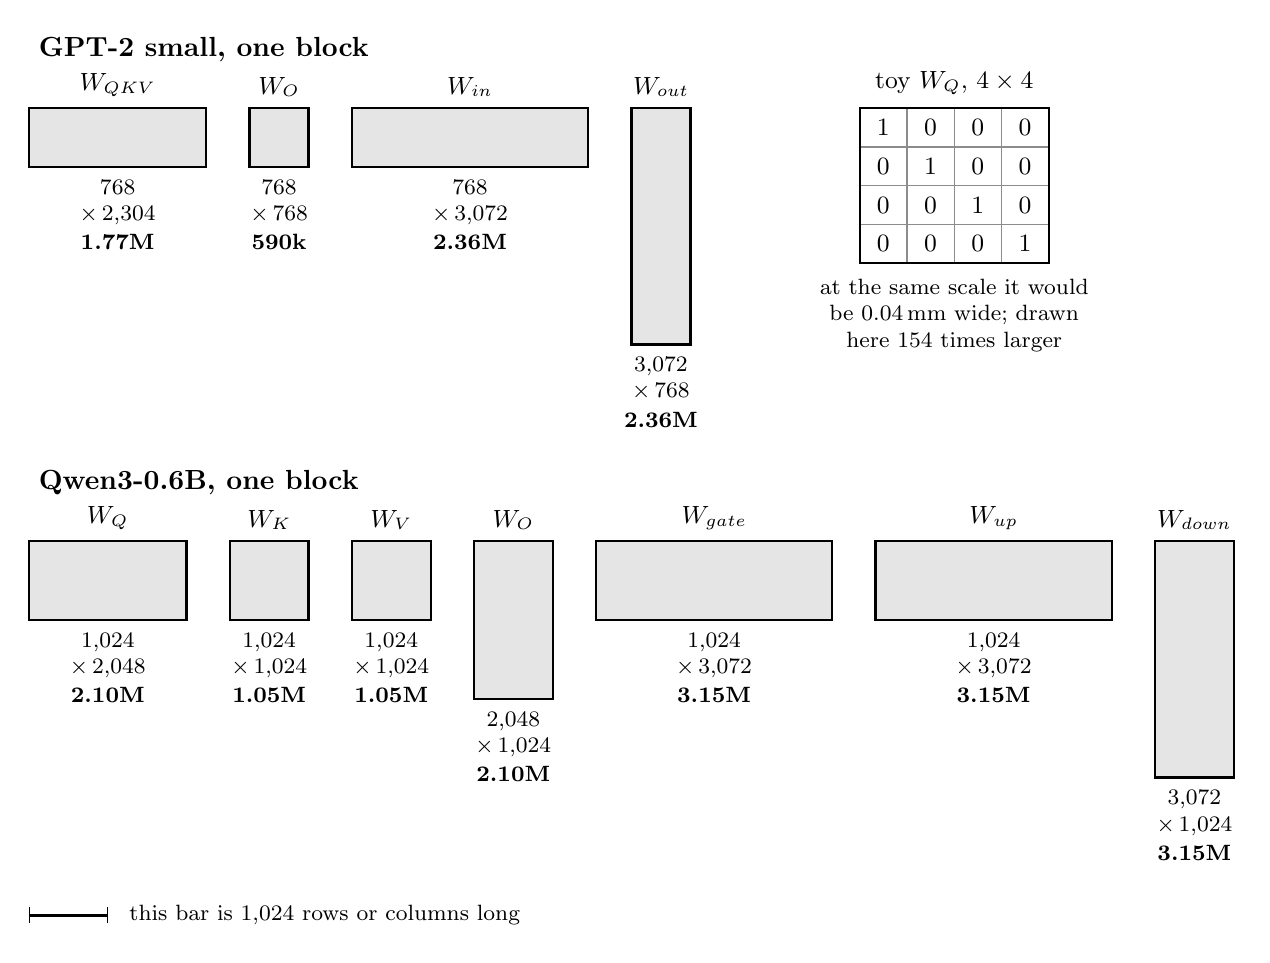
\begin{tikzpicture}
\node[anchor=west, font=\normalsize\bfseries] at (0,0.75) {GPT-2 small, one block};
\draw[line width=0.8pt, fill=black!10] (0.000,0.000) rectangle (2.250,-0.750);
\node[anchor=south, font=\small] at (1.125,0.020) {$W_{QKV}$};
\node[anchor=north, font=\footnotesize, align=center] at (1.125,-0.790) {768\\$\times$\,2{,}304\\[1pt]\textbf{1.77M}};
\draw[line width=0.8pt, fill=black!10] (2.800,0.000) rectangle (3.550,-0.750);
\node[anchor=south, font=\small] at (3.175,0.020) {$W_O$};
\node[anchor=north, font=\footnotesize, align=center] at (3.175,-0.790) {768\\$\times$\,768\\[1pt]\textbf{590k}};
\draw[line width=0.8pt, fill=black!10] (4.100,0.000) rectangle (7.100,-0.750);
\node[anchor=south, font=\small] at (5.600,0.020) {$W_{\text{in}}$};
\node[anchor=north, font=\footnotesize, align=center] at (5.600,-0.790) {768\\$\times$\,3{,}072\\[1pt]\textbf{2.36M}};
\draw[line width=0.8pt, fill=black!10] (7.650,0.000) rectangle (8.400,-3.000);
\node[anchor=south, font=\small] at (8.025,0.020) {$W_{\text{out}}$};
\node[anchor=north, font=\footnotesize, align=center] at (8.025,-3.040) {3{,}072\\$\times$\,768\\[1pt]\textbf{2.36M}};
\draw[black!45, fill=white] (10.550,0.000) rectangle (11.150,-0.492);
\node[font=\small, text=black] at (10.850,-0.246) {$1$};
\draw[black!45, fill=white] (11.150,0.000) rectangle (11.750,-0.492);
\node[font=\small, text=black] at (11.450,-0.246) {$0$};
\draw[black!45, fill=white] (11.750,0.000) rectangle (12.350,-0.492);
\node[font=\small, text=black] at (12.050,-0.246) {$0$};
\draw[black!45, fill=white] (12.350,0.000) rectangle (12.950,-0.492);
\node[font=\small, text=black] at (12.650,-0.246) {$0$};
\draw[black!45, fill=white] (10.550,-0.492) rectangle (11.150,-0.984);
\node[font=\small, text=black] at (10.850,-0.738) {$0$};
\draw[black!45, fill=white] (11.150,-0.492) rectangle (11.750,-0.984);
\node[font=\small, text=black] at (11.450,-0.738) {$1$};
\draw[black!45, fill=white] (11.750,-0.492) rectangle (12.350,-0.984);
\node[font=\small, text=black] at (12.050,-0.738) {$0$};
\draw[black!45, fill=white] (12.350,-0.492) rectangle (12.950,-0.984);
\node[font=\small, text=black] at (12.650,-0.738) {$0$};
\draw[black!45, fill=white] (10.550,-0.984) rectangle (11.150,-1.476);
\node[font=\small, text=black] at (10.850,-1.230) {$0$};
\draw[black!45, fill=white] (11.150,-0.984) rectangle (11.750,-1.476);
\node[font=\small, text=black] at (11.450,-1.230) {$0$};
\draw[black!45, fill=white] (11.750,-0.984) rectangle (12.350,-1.476);
\node[font=\small, text=black] at (12.050,-1.230) {$1$};
\draw[black!45, fill=white] (12.350,-0.984) rectangle (12.950,-1.476);
\node[font=\small, text=black] at (12.650,-1.230) {$0$};
\draw[black!45, fill=white] (10.550,-1.476) rectangle (11.150,-1.968);
\node[font=\small, text=black] at (10.850,-1.722) {$0$};
\draw[black!45, fill=white] (11.150,-1.476) rectangle (11.750,-1.968);
\node[font=\small, text=black] at (11.450,-1.722) {$0$};
\draw[black!45, fill=white] (11.750,-1.476) rectangle (12.350,-1.968);
\node[font=\small, text=black] at (12.050,-1.722) {$0$};
\draw[black!45, fill=white] (12.350,-1.476) rectangle (12.950,-1.968);
\node[font=\small, text=black] at (12.650,-1.722) {$1$};
\draw[line width=0.9pt] (10.550,0.000) rectangle (12.950,-1.968);
\node[anchor=south, font=\small, align=center] at (11.750,0.05) {toy $W_Q$, $4\times4$};
\node[anchor=north, font=\footnotesize, align=center, text width=4.6cm] at (11.750,-2.048) {at the same scale it would be 0.04\,mm wide; drawn here 154 times larger};
\node[anchor=west, font=\normalsize\bfseries] at (0,-4.75) {Qwen3-0.6B, one block};
\draw[line width=0.8pt, fill=black!10] (0.000,-5.500) rectangle (2.000,-6.500);
\node[anchor=south, font=\small] at (1.000,-5.480) {$W_Q$};
\node[anchor=north, font=\footnotesize, align=center] at (1.000,-6.540) {1{,}024\\$\times$\,2{,}048\\[1pt]\textbf{2.10M}};
\draw[line width=0.8pt, fill=black!10] (2.550,-5.500) rectangle (3.550,-6.500);
\node[anchor=south, font=\small] at (3.050,-5.480) {$W_K$};
\node[anchor=north, font=\footnotesize, align=center] at (3.050,-6.540) {1{,}024\\$\times$\,1{,}024\\[1pt]\textbf{1.05M}};
\draw[line width=0.8pt, fill=black!10] (4.100,-5.500) rectangle (5.100,-6.500);
\node[anchor=south, font=\small] at (4.600,-5.480) {$W_V$};
\node[anchor=north, font=\footnotesize, align=center] at (4.600,-6.540) {1{,}024\\$\times$\,1{,}024\\[1pt]\textbf{1.05M}};
\draw[line width=0.8pt, fill=black!10] (5.650,-5.500) rectangle (6.650,-7.500);
\node[anchor=south, font=\small] at (6.150,-5.480) {$W_O$};
\node[anchor=north, font=\footnotesize, align=center] at (6.150,-7.540) {2{,}048\\$\times$\,1{,}024\\[1pt]\textbf{2.10M}};
\draw[line width=0.8pt, fill=black!10] (7.200,-5.500) rectangle (10.200,-6.500);
\node[anchor=south, font=\small] at (8.700,-5.480) {$W_{\text{gate}}$};
\node[anchor=north, font=\footnotesize, align=center] at (8.700,-6.540) {1{,}024\\$\times$\,3{,}072\\[1pt]\textbf{3.15M}};
\draw[line width=0.8pt, fill=black!10] (10.750,-5.500) rectangle (13.750,-6.500);
\node[anchor=south, font=\small] at (12.250,-5.480) {$W_{\text{up}}$};
\node[anchor=north, font=\footnotesize, align=center] at (12.250,-6.540) {1{,}024\\$\times$\,3{,}072\\[1pt]\textbf{3.15M}};
\draw[line width=0.8pt, fill=black!10] (14.300,-5.500) rectangle (15.300,-8.500);
\node[anchor=south, font=\small] at (14.800,-5.480) {$W_{\text{down}}$};
\node[anchor=north, font=\footnotesize, align=center] at (14.800,-8.540) {3{,}072\\$\times$\,1{,}024\\[1pt]\textbf{3.15M}};
\draw[line width=1pt] (0,-10.25) -- (1,-10.25); \draw (0,-10.15) -- (0,-10.35) (1,-10.15) -- (1,-10.35); \node[anchor=west, font=\footnotesize] at (1.15,-10.25) {this bar is 1{,}024 rows or columns long};
\end{tikzpicture}}
